\chapter{Genome assembly of \textit{Gemmata} isolates}
\label{chap:assembly}

\section{Preface}
This chapter and appendix x briefly describe my work on two genome sequencing projects during my time at the University of Canterbury. This work describes the genome assembly and preliminary analysis of \textit{Gemmata} isolates, as part of a collaboration with Paul Gardner, Amy Osborne and Anthony Poole. This builds on previous work in this group, which explored the relationship between expression of ncRNAs and phylogenetic distance, which concluded that phylogeny-informed sampling is required for comparative methods to be effective. For this project, outgroups in the 'goldilocks zone', i.e phyla at a specific distance that will allow transcriptomic comparison, including \textit{Gemmata}, have been selected for sequencing. 

\section{Contributions}
I performed all assembly and data analysis. Isolates were grown and prepared for sequencing by Amy Osborne.
\newpage
\section{Introduction}

\textit{Gemmata} are a genus of aerobic budding bacteria found in freshwater and in soil, which is of particular interest in evolutionary biology due to their phenotypic similarity to eukaryotes and archaea \citep{Franzmann1984-ms,Devos2013-ds}. \textit{Gemmata} are part of the Planctomycetes superphylum, which are a widespread group of environmental bacteria with unusual phenotypic and physiological characteristics reminiscent of eukaryotic cell. An especially noteable feature of planctomycetes is the presence of intracellular compartments \citep{Lindsay2001-qg}, including a large compartment enclosing the nucleoid that has been found in \textit{Gemmata obscuriglobus} (Figure \ref{fig:gemmata_cell}) \citep{Fuerst2005-kx}. 

\begin{figure}[H]
    \begin{minipage}{0.7\textwidth}
    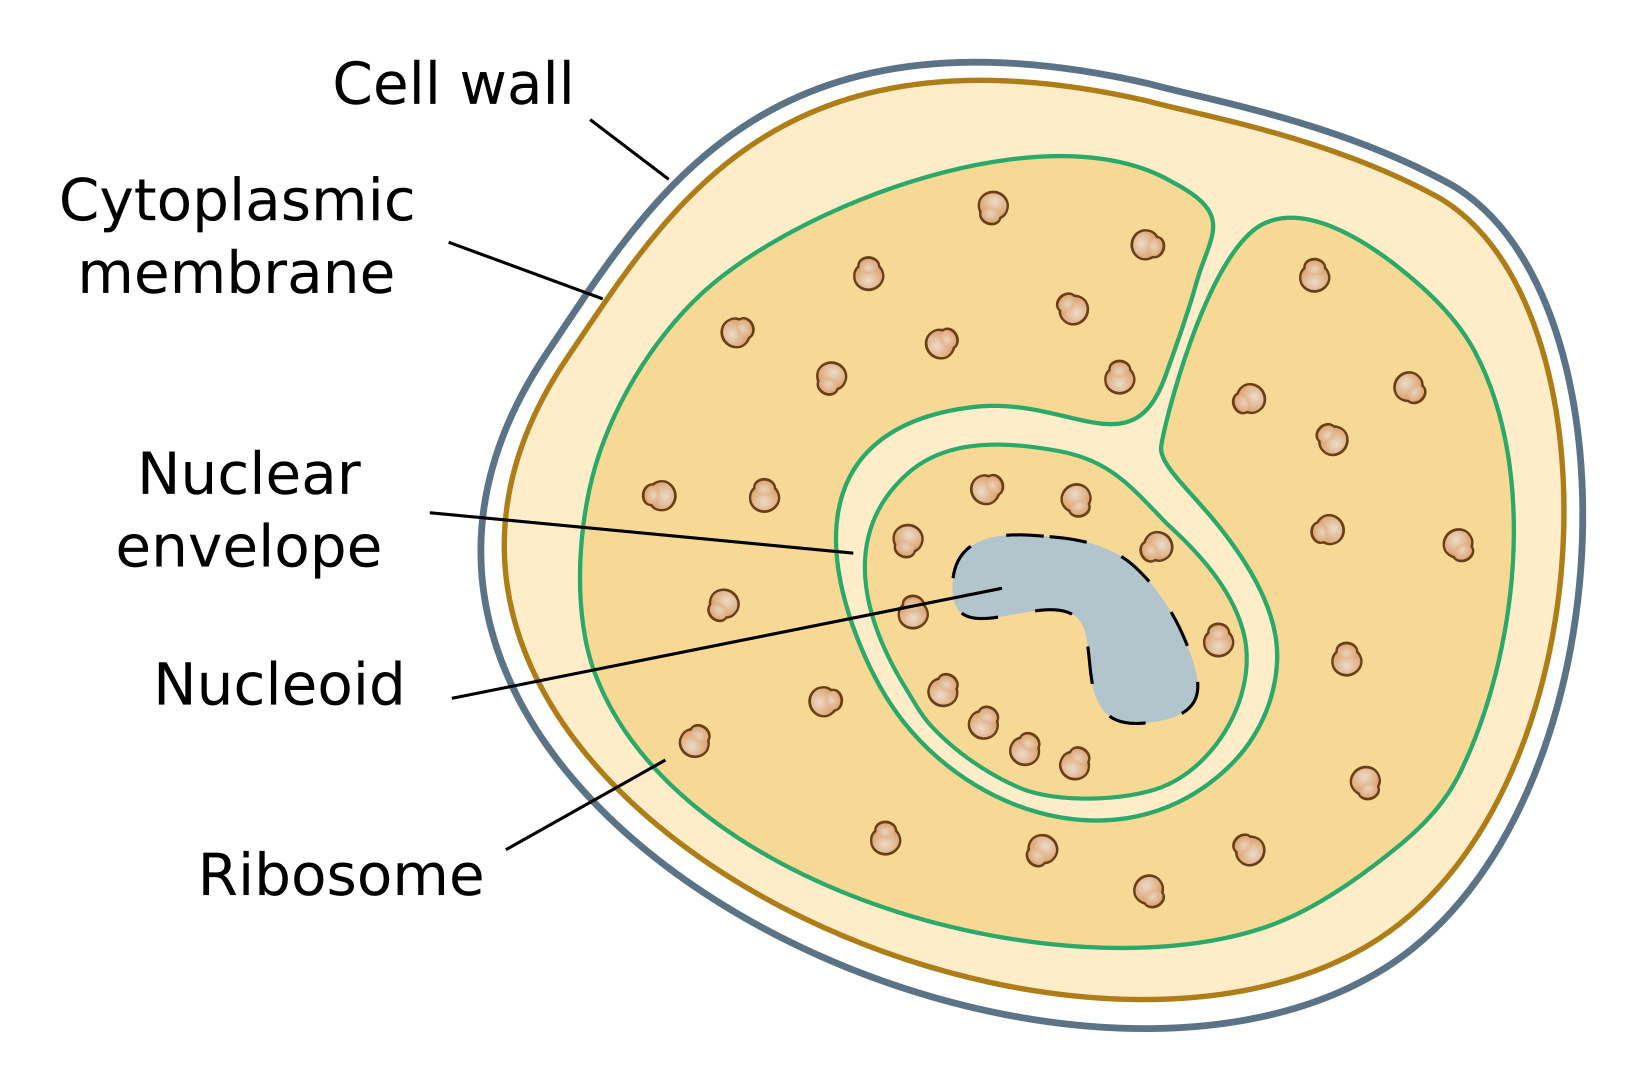
\includegraphics[scale=0.7]{assembly/gemmata_cell.png}
    \end{minipage}
    \begin{minipage}{0.29\textwidth}
    \caption[Diagram showing the intracellular compartments of a \textit{Gemmata obscuriglobus} cell]{Diagram showing the intracellular compartments of a \textit{Gemmata obscuriglobus} cell. Adapted from \cite{Fuerst2011-le}.}
    \label{fig:gemmata_cell}
    \end{minipage}
\end{figure}

The taxonomic placement of planctomycetes has been debated, as they share phenotypic features with eukaryotes, such as reproduction \textit{via} yeast-like budding of the extracellular membrane, and also contain ammonia metabolic pathways normally found in archaea \citep{Fuchsman2006-zz,Fuerst2011-le}. \textit{Gemmata obscuriglobus} also has the unusual ability produce sterols \citep{Rivas-Marin2019-jd}, and utilises an endocytosis-like system for protein uptake \citep{Lonhienne2010-qa}.

However, there is some debate as to whether these features are structurally analagous rather than due to some shared homology \citep{McInerney2011-bx}. Planctomycetes have no substantial shared gene content with other kingdoms, aside from some small amount presumably obtained by HGT \citep{Fuchsman2006-zz}.

Currently, only a handful of representative strains and genome sequences are available for \textit{Planctomycetes}, with \textit{G. obscuriglobus} being the sole sequenced representative of the genus \textit{Gemmata}. We have sequenced and annotated the genomes of a strain of \textit{G. obscuriglobus}, and 4 other \textit{Gemmata}-like isolates as part of an effort to increase the number of genomes available for comparison for this under-sampled bacterial phyla \citep{Wu2009-zh}. 
This chapter describes the assembly, annotation and a preliminary comparative analysis of these genomes, which found large numbers of transposons in \textit{G. obscuriglobus}, and high levels of rearrangements across the clade.

\section{Methods}

\subsection{Sequencing}
\textit{Gemmata} isolates were collected from Queensland, Australia. \textit{Gemmata}-like str. JW3-9s0 (aka Soil9) and \textit{Gemmata obscuriglobus} were isolated from soil, \textit{Gemmata}-like str. CJuq14 and \textit{Gemmata}-like str. JW9-3f1 from a eutrophic lake and \textit{Gemmata}-like str. JW11-2f5 from an ornamental fountain. Isolates were previously classified as Gemmata-like based on phylogenetic analysis of 16S sequences \citep{Wang2002-qh}. Samples were isolated, cultured and prepared for sequencing as described in \citep{Wang2002-qh}. The genomes of all isolates were sequenced using Pacific Biosciences SMRT$\textsuperscript{TM}$ sequencing. 

\subsection{Assembly and analysis}

Raw bas.h5 files were converted to fastq reads with bash5tools.py from the pbh5tools package from PacificBiosciences (https://github.com/PacificBiosciences/pbh5tools/). Reads were trimmed and assembled using Canu v1.5 (default settings) \citep{Koren2017-fv}. Genomes were circularised with Circlator \citep{Hunt2015-tj}. Reads were mapped to the genome assemblies using BLASR \citep{Chaisson2012-sx} to generate alignments for Qualimap, which was used to assess coverage and quality of the assemblies \citep{Okonechnikov2016-ly}. Genome assemblies were annotated with Prokka \citep{Seemann2014-sxxa}. To improve gene annotations, a custom database of planctomycetes protein annotations was used as an additional reference, consisting of all protein annotations of plantomycete genomes from NCBI. The gram negative option for identifying signal peptides was used during annotation, as genes involved in outer membrane biogenesis have previously been identified in \textit{Planctomycetes} \citep{Speth2012-of}. Whole genome alignments were performed using mauve genome aligner \citep{Darling2010-vl}. Roary was used to identify the number of orthologous genes between the isolates \citep{Page2015-lu}. 

\section{Results and Discussion}

The genome assembly tools completely resolved two genomes, \textit{G. obscuriglobus} UQM2246 and \textit{Gemmata}-like str. JW11, and generated large high-coverage contigs for other strains (Table \ref{tab:genome_stats}). The genome sizes ranged between 7.86--10.14 Mb, with high \% GC content (64--70\%), which is consistent with the genomes of other \textit{Gemmata} and \textit{Planctomycete} genomes \citep{Franke2018-ys}. A small contig in the \textit{Gemmata}-like str. CJuql4 assembly was classed as a plasmid by Circlator. Plasmid-encoded RepA proteins were annotated in larger contigs in Gemmata-like str. JW9 and Gemmata-like str. JW3-8s0, indicating that plasmid reads may have been mis-assembled into genome contigs. CRISPR-cas casettes were also detected in all assemblies except \textit{Gemmata}-like str. JW9, however \textit{cas} endonucleases were found in all genome assemblies (Table \ref{tab:annotation_stats}).

\begin{table}[H]
    \footnotesize
    \centering
\begin{tabular}{rcccccc}\toprule
Strain & Genome Contigs & Size (Mb) & \% GC &
Circular & Plasmid contigs & Mean coverage (X)\\
\midrule
UQM2246 & 1 & 8.99 & 67.36 & Yes & 0 & 106  \\
JW3-8s0 & 1 & 10.14 & 63.95 &  No & 0 & 91\\
CJuql4 & 3 & 7.94 & 69.87 & No & 1 & 109\\
JW11 & 1 & 8.86 &  68.71 & Yes & 0 & 91\\
JW9 & 5 & 10.03 & 64.14 & No & 0 & 96 \\
\bottomrule
    \end{tabular}
    \caption[Summary of \textit{Gemmata} genome assemblies]{Summary of \textit{Gemmata} genome assemblies, percentage GC content, predicted plasmid contigs, and coverage.}
    \label{tab:genome_stats}
\end{table}

\begin{table}[H]
    \footnotesize
    \centering
\begin{tabular}{rccccccp{1.2cm}p{1.2cm}p{1.15cm}}\toprule
Strain & Genes & CDS & rRNA & tRNA & tmRNA & misc RNA & Signal peptides & CRISPR regions & Cas proteins\\
\midrule
UQM2246 & 7824 & 7702 & 12 & 101 & 1 & 8 & 912 & 4 & 1, 2, 3, 4, 6, 7\\
JW3-8s0 & 8994 & 8883 & 9 & 101 & 1 & - & 1075 & 4 & 1, 2, 3, 4 \\
CJuql4 & 7115 & 6984 & 6 & 110 & 1 & 14 & 959 & 1 & 1, 2, 4\\
JW11 & 8003 & 7885 & 6 & 94 & 1 & 17 & 961 & 2 & 1, 2, 3, 4, 5, 6, 7, 8\\
JW9 & 9344 & 9213 & 6 & 114 & 1 & 10 & 1016 & - & 1, 2, 4\\
\bottomrule
    \end{tabular}
    \caption[Summary of Prokka genome annotations for \textit{Gemmata} genome assemblies]{Summary of Prokka genome annotations for \textit{Gemmata} genome assemblies.}
    \label{tab:annotation_stats}
\end{table}

Whole-genome alignments of the genome assemblies showed the \textit{Gemmata} genomes have highly diverse genome structures (Figure \ref{fig:mauve}), despite high overall shared gene content. Previous estimates based on 16S sequences that \textit{Gemmata}-like isolates JW9, Cjuql4 and JW3-8s0 are strains of a single \textit{Gemmata} species \citep{Wang2002-qh}. A pan-genome \texttt{Roary} analysis found that 633 genes were shared between all 5 strains, and 21986 genes were unique to a single genome. These consisted of uncharacterised hypothetical proteins, and components of mobile genetic elements. The accessory gene tree (Figure \ref{fig:roary_tree}), showing the similarity between cohorts of accessory genes between strains, also reflects the relationships shown in 16S tree produced here and by \cite{Wang2002-qh}.

Protein annotation found that all genome assemblies contain high numbers of mobile genetic elements (Table \ref{tab:gemmata_MGEs}), with \textit{G. obscuriglobus} containing 217 predicted transposases. The true number of these elements may be larger, as many predicted proteins were not able to be functionally annotated. 

%this study found lipopolysachs \citep{Mahat2016-gh} \citep{Sagulenko2014-ho} Although the structure of the outer membrane of Gemmata species is debated \citep{Sagulenko2014-ho}, lipopolysaccharides have recently been identified in \textit{G. obscuriglobus} \citep{Mahat2016-gh}. planctos....databases will increase and better annotations %In any case the proposal of Gram-negativity of the planctomycete wall and consequent rejection of the paryphoplasm depends at present solely on genomic evidence suggesting presence of such genes as those for lipid A synthesis and outer membrane proteins [33], but the location of relevant gene products in any planctomycete has not yet been determined. So such bioinformatic analysis can have no definite implications for interpretation of cell structure and can easily lead to misinterpretation without further localization evidence.%

\begin{figure}[H]
    \centering
    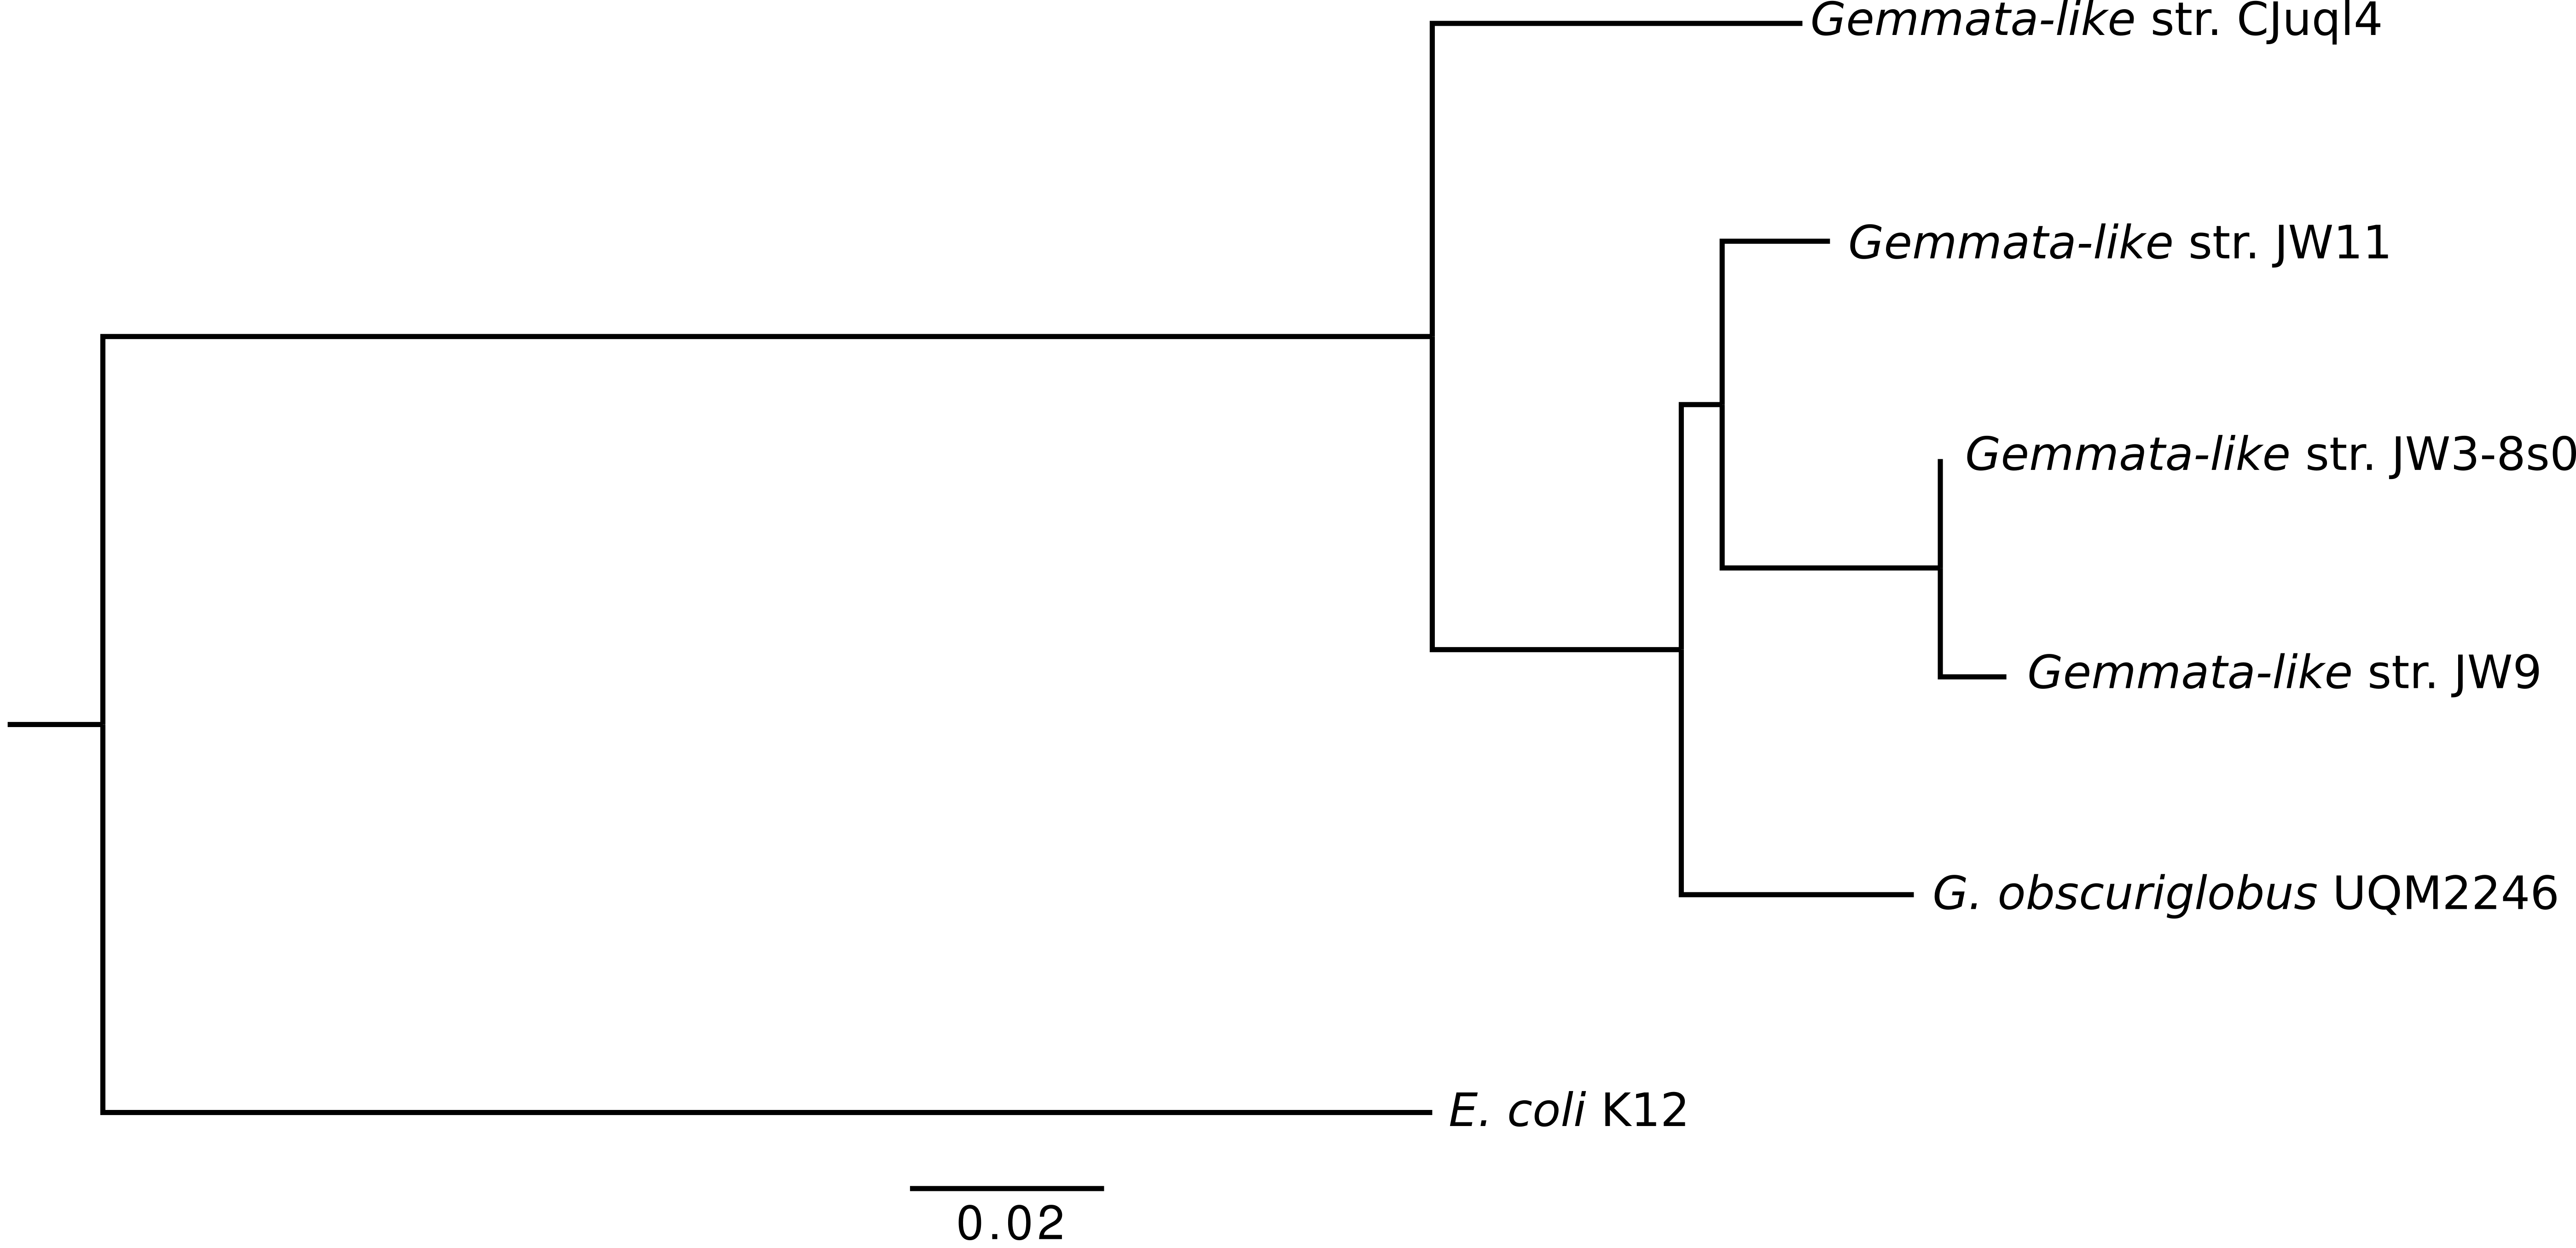
\includegraphics[scale=0.17]{assembly/gem_16S.png}
    \caption[16S tree of \textit{Gemmata} genome assemblies]{16S tree of \textit{Gemmata} genome assemblies, with E. coli K12 included as an outgroup. 16S sequences annotated by Prokka were aligned to a 16S covariance model sequences from Rfam. The \textit{E. coli} K12 sequence was also included as an outgroup. Phylogenetic tree was generated by ClustalW2 (distance correction=on, type=neighbour-joining). Figure generated in Figtree ($https://github.com/rambaut/figtree$)}
    \label{fig:my_label}
\end{figure}

\begin{figure}
    \centering
    
\includegraphics[scale=0.3]{assembly/accessory_tree.png}
    \caption[Accessory gene tree for \textit{Gemmata} genome assemblies]{Phylogeny showing the relationships between the \textit{Gemmata} genome assemblies based on gene content. Tree generated by \texttt{Roary} \citep{Page2015-lu} and visualised in Figtree.}
    \label{fig:roary_tree}
\end{figure}

\begin{figure}[H]
    \centering
    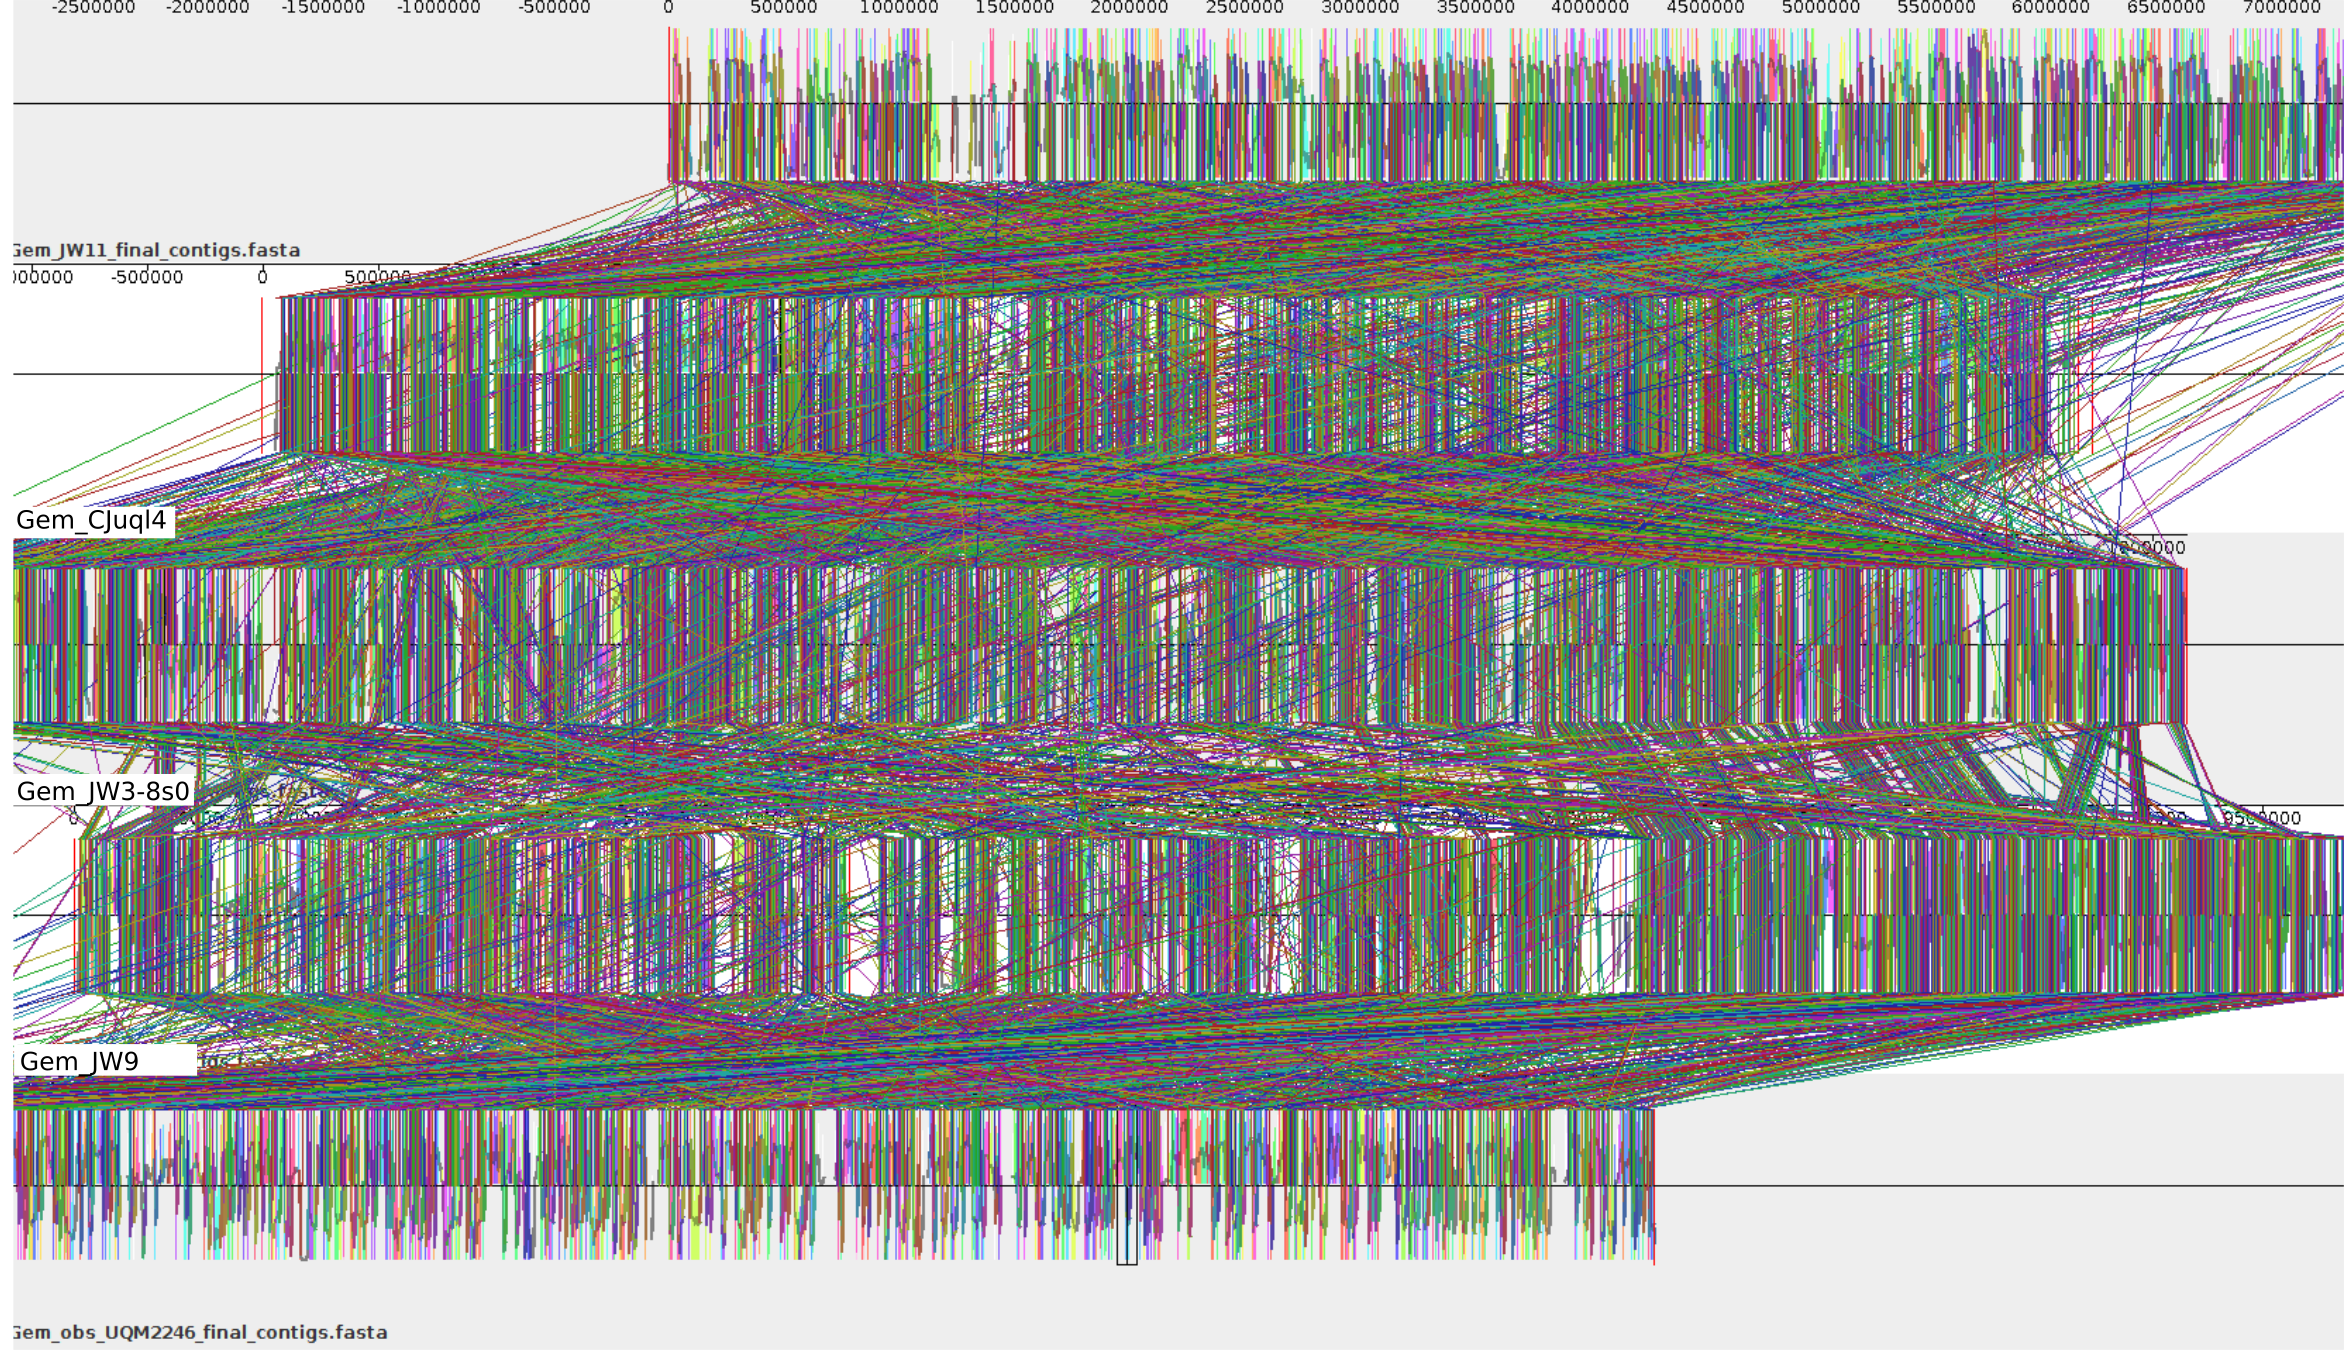
\includegraphics[scale=0.8]{assembly/mauve.png}
    \caption[Overview of the mauve alignment of the \textit{Gemmata} genome assemblies]{Overview of the mauve alignment of the \textit{Gemmata} genome assemblies. Local colinear blocks, consisting of shared sequence regions throughout the genomes, are shown as different colours and linked by connecting lines. This alignment shows extremely high levels of rearrangement between these genomes, despite high amount of shared gene content.}
    \label{fig:mauve}
\end{figure}

\begin{table}[H]
    \footnotesize
    \centering
\begin{tabular}{cccccc}\toprule
Annotation & CJuql4 & JW3-8s0 & JW11 & JW9 & UQM2246\\\midrule
Transposase & 36 & 88 & 67 & 81 & 217 \\
Integrase & 11 & 6 & 18 & 6 & 4\\
Recombinase & 12 & 36 & 10 & 37 & 22 \\
Prophage-like regions & 4 & 3 & 4 & 3 & 7 \\
\bottomrule
    \end{tabular}
    \caption[Summary of mobile genetic element annotations in \textit{Gemmata} genome assemblies]{Summary of mobile genetic element annotations in \textit{Gemmata} genome assemblies. Total number of proteins annotated as `transposase', `integrase' or `recombinase' in the prokka annotations are shown for each genome. Prophage-like regions refers to the total number of predicted prophage containing regions generated by PHAST \citep{Zhou2011-es}.}
    \label{tab:gemmata_MGEs}
\end{table}

The remarkably high level of rearrangements in these genomes may be due to the high numbers of mobile genetic elements in these genomes (Table \ref{tab:gemmata_MGEs}). This is likely in part due to the large size of \textit{Gemmata} genomes, as genome size is thought to be the largest contributor for both the overall number and density of insertion sequence (IS) elements \citep{Touchon2007-an}. 

High levels of rearrangements associated with IS density have been found in various linages in Cyanobacteria \citep{Bhaya2007-zk}. Evidence that certain IS families are under positive selection in the ammonia-fixing cyanobacterium \textit{Crocosphaera watsonii}, indicates that tranposition can provide a selective advantage in organisms living in similar oligotrophic environments and with similar genome sizes to \textit{Gemmata} sp. . \citep{Kaneko2007-qp} have suggested that lifestyle adaption may play a part in copy-number expansion in the Cyanobacteria \textit{Microcystis aeruginosa}, which contains 452 ISs compared to < 100 in other related genera, as mutations and rearrangements associated with transposition were also enriched in the genome.

Rapid expansion of transposons has been also been observed in the genomes of \textit{Salinivibrio} symbionts in anglerfish, in which 28-31\% of the coding sequences are transposase genes, compared to 2\% in their non-symbiont counterparts \citep{Hendry2018-vk}. High transposon copy-number has been found in the genomes of Baltic Sea Cyanobacteria. The enrichment of transposase transcripts in ocean metagenomes suggests that these are also actively expressed. It has been is suggested that these transposons provide can accelerate certain evolutionary processes, by providing genomic plasticity and hence an adaptive advantage in changeable coastal environments \citep{Vigil-Stenman2017-yz}

Other examples of MGE enrichment can also be found in slow-growing free-living bacteria and symbionts \citep{Vigil-Stenman2015-et,Schmitz-Esser2011-ss}. The unusual budding mode of reproduction and slow growth of \textit{Gemmata} species may reduce their capacity to expunge such elements. An analagous example are the asexually reproducing eukaryotes such as bdelloid rotifers, which have developed additional defences to reduce transposon activity \citep{Flot2013-cg} and prevent deleterious proliferation of transposons \citep{Arkhipova2005-me}.  

%Gemmata-like str. CJuq-L4	121115	Gemmata	11772655	AF239693		eutrophic lake
%Gemmata-like str. Soil9	121120	Gemmata	11772655	AF239698		Charles Crossing Rd. soil
%Gemmata-like str. JW11-2f5	121118	Gemmata	11772655	AF239696		ornamental fountain
%Gemmata-like str. JW3-8s0	121116	Gemmata	11772655	AF239694		Mt. Coot-tha soil
%Gemmata-like str. JW9-3f1	121119	Gemmata	11772655	AF239697		eutrophic lake

\section{Future Directions}
This chapter describes the genome assembly, annotation and a preliminary comparative analysis of five \textit{Gemmata} isolates. These genomes are enriched in mobile genetic elements, and appear to have highly dynamic genome structures. Future work aims to generate transcriptomes of these strains, with the primary aim of annotating novel ncRNAs as part of a follow-on to work by \cite{Lindgreen2014-plplvr}. This project also includes the assembly of \textit{Halococcus} genomes, which I have also assembled and annotated (unpublished data). 

These genomes also provide a resource for further study of the enigmatic\textit{ Planctomycetes} bacteria, in particular the genomic basis for the eukaryotic and archaea-like phenotypes observed in \textit{Gemmata} strains. Additional annotation of these \textit{Gemmata} genomes is required to further characterise MGEs, and identify if these are active, and identify the mechanisms behind the apparent high rate of recombination in these genomes. These genomes also appear to replicate the previous observations of high transposon copy-number in bacteria living in complex aquatic environments, suggesting that transposon copy-number may provide an adaptive advantage in these environments. 

\bibliographystyle{otago}
\bibliography{assembly}
